%!TEX TS-program = xelatex
%!TEX encoding = UTF-8 Unicode

\documentclass[a4paper, 11pt]{article}
\usepackage{amsmath}
\usepackage{amsfonts}
\usepackage{graphicx}
\usepackage{fontspec}
\usepackage{xunicode}
\usepackage{xcolor}
\usepackage{wrapfig}
\usepackage[margin=0.8in]{geometry}

\usepackage{sectsty}
\usepackage{titlesec}
\usepackage{multicol}

\setmainfont{sylfaen.ttf}

\setlength{\parindent}{0pt}
\setlength{\parskip}{1.5ex plus 0.5ex minus 0.5ex}
\setlength{\abovedisplayskip}{2.5ex}
\setlength{\belowdisplayskip}{2.5ex}
\setlength{\abovedisplayshortskip}{1.5ex}
\setlength{\belowdisplayshortskip}{1.5ex}

\allsectionsfont{\large\addfontfeatures{FakeBold}}
\titlespacing\section{0pt}{5.0ex plus 0.5ex minus 0.5ex}{1.5ex plus 0.5ex minus 0.5ex}

\newcommand{\setN}{\mathbb{N}}
\newcommand{\setZ}{\mathbb{Z}}

\definecolor{alt}{RGB}{102, 102, 0}

\begin{document}
\begin{sloppypar}

\begin{center}
\Large
{
\addfontfeatures{FakeBold}
დისკრეტული მათემატიკა
}

\large
ამოცანების ამოხსნები \#20

\normalsize
\hfill მოამზადა მარიამ წიქარიშვილმა
\end{center}

\section{კონსპექტის ამოცანა 10.24(გვ. 203)}

\textbf{\textcolor{red}{ლათინური კვადრატი}} ეწოდება ისეთ $n\times n$ უჯრიან კვარდატს, რომელშიც ყველა უჯრაში 1-დან n-მდე რამე მთელი რიცხვი ისე წერია, რომ ყოველ სვეტში და ყოველ სტრიქონში 1-დან n-მდე ყველა რიცხვი ზუსტად ერთხელ გვხვდებოდეს.

ა) გვ 205-ზე მოცემულია ნაწილობრივ შევსებული ლათინური კვარდატი(ე.წ. ლათინური მართკუთხედი). შეავსეთ ამ კვადრატის დარჩენილი ორი სტრიქონი.

ბ) აჩვენეთ, რომ ლათინური მართკუთხედის შემდეგი სტრიქონის შევსების ამოცანა რომელიღაც $2*n$ წვეროიან ორნაწილიან გრაფში დაწყვილების პოვნის ამოცანის ექვივალენტურია.

გ) დაამტკიცეთ, რომ (ბ) პუნქტში შედგენილ ამოცანაში დაწყვილება ყოველთვის იარსებებს და შესაბამისად დაასკვენით, რომ ნებისმიერი ლათინური მართკუთხედი შეგვიძლია ლათინურ კვადრატამდე შევავსოთ.

{
\addfontfeatures{FakeBold}
ამოხსნა:
}

ა) ჯერ შევავსოთ მე-4 სტრიქონი, შემდეგ კი მე-5. თითო სვეტსა და სტრიქონში თითოეული რიცხვი უნდა გვხვდებოდეს ერთადერთხელ, ამიტომ მეოთხე სტრიქონის შევსებამდე დავაკვირდეთ თითოეულ სვეტში რომელი ციფრები გვაქვს გამოუყენებელი(შესაბამისად ახლა ჩაწერა შეგვიძლია). ესენია პირველიდან მეხუთე სვეტამდე, შესაბამისად $\{1 , 5\}$, $\{3,5\}$, $\{2,4\}$, $\{1,4\}$ და $\{2,3\}$. არ აქვს მნიშვნელობა მე-4 სტრიქონში ამ ორიდან რომელ მნიშვნელობას ავირჩევთ(გაგრძლებება მაინც შეგვეძლება), რამდენადაც ეს 2 მნიშვნელობა 2 უჯრაზე უნდა გადანაწილდეს.(სულაც შეგვიძლია სტრიქონებს ადგილები გავუცვალოთ და მაინც იქნება ლათინური კვადრატი). ამრიგად, მე-4 სტრიქონის 1-ლი სვეტისთვის ავიჩიოთ ორიდან ნებისმიერი მნიშვნელობა. ასე გავაგრძელოთ, მთავარია შემდეგი წყვილებიდან არ ავირჩიოთ ისეთი მნიშვნელობები, რომელიც ამ სტრიქონში უკვე გამოვიყენეთ. მე-5 სტრიქონში წყვილიდან დარჩენილებს ჩავწერთ და აღმოჩნდება, რომ კორექტულად შეივსო.
\begin{center}
\begin{tabular}{|c|c|c|c|c|} 
    \hline
    $2$ & $4$ & $5$ & $3$ & $1$ \\
    \hline 
    $4$ & $1$ & $3$ & $2$ & $5$ \\
    \hline
    $3$ & $2$ & $1$ & $5$ & $4$ \\
    \hline
    $1$ & $5$ & $2$ & $4$ & $3$ \\
    \hline 
    $5$ & $3$ & $4$ & $1$ & $2$ \\
    \hline 
\end{tabular}
\end{center}

შეიძლება გვეგონოს, რომ მე-5 სტრიქონის სწორად შევსება შემთხვევითიაა, თუმცა ეს ასე არაა, რასაც შემდეგ ნაწილებში დავამტკიცებთ.

ბ) დავუშვათ, გვაქვს $n\times n$-ზე ლათინური კვადრატი, რომლის პირველი $k$ სტრიქონი სწორადაა შევსებული. $(k+1)$-ე სტრიქონის შევსებისას $n$ რიცხვი გვაქვს, რომელიც $n$ პოზიციაზე უნდა ჩავწეროთ (სტრიქონში ყველა რიცხვი უნდა ეწეროს, თან თითოჯერ). ანუ ჩვენი ამოცანა იგივეა, რაც პოზიციას (სვეტის ნომერს) შევუსაბამოთ $1$-დან $n$-მდე რიცხვი, ოღონდ ისე რომ სვეტი არ დავაწყვილოთ რიცხვთან, რომელიც უკვე არის ამ სვეტში. გვაქვს $2*n$ წვეროიან ორნაწილიან გრაფი, რომლის ერთ მხარეს გვაქვს სვეტის ნომრები, მეორე მხარეს $1$-დან $n$-მდე რიცხვები, ასევე წიბოები(რომელი სვეტის რომელ ციფრთან დაწყვილება შეიძლება აღნიშნულია წიბოთი) და უნდა ვიპოვოთ მათ შორის შესაბამისობა (რომელი რიცხვი სად ჩაიწერება) ანუ უნაკლო დაწყვილება ამ წიბოების ფარგლებში.

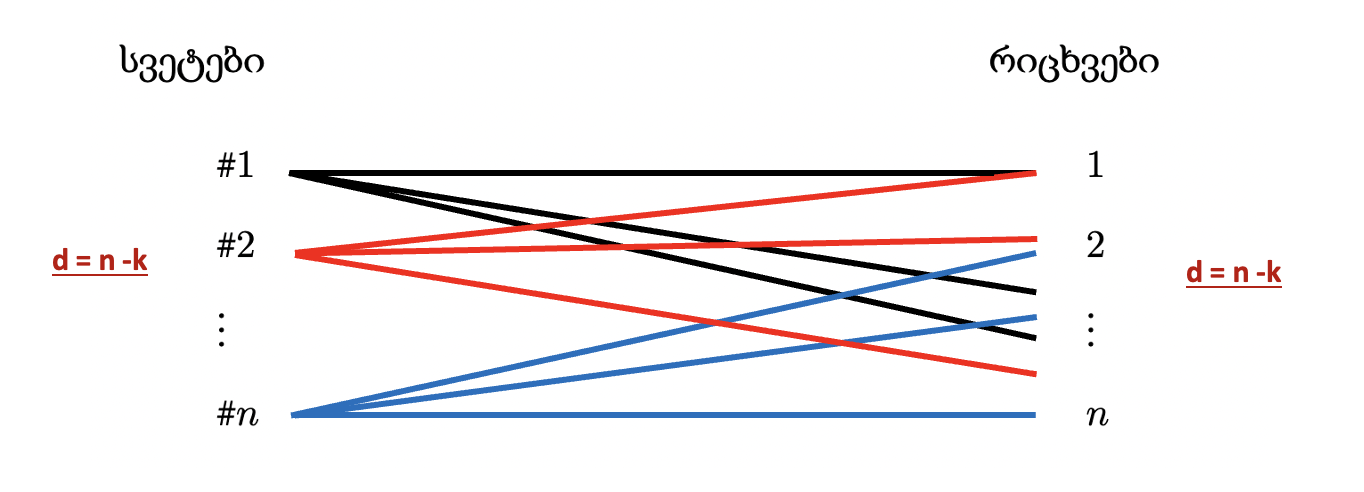
\includegraphics[scale = 0.7]{1.png}
% ჯერ ასე ავაგე სიები მაგრამ შემდეგ წიბოები ვერ გავავლე და ამიტომ სხვაგან გავაკეთე და სურათი ჩავსვი
% \begin{multicols}{2}
% სვეტები
% \begin{enumerate}
%   \item[] $\#1$
%   \item[] $\#2$
%   \item[] $\vdots$
%   \item[] $\#n$
% \end{enumerate}

% \columnbreak

% რიცხვები
% \begin{enumerate}
%   \item[] $1$
%   \item[] $2$
%   \item[] $\vdots$
%   \item[] $n$
% \end{enumerate}
% \end{multicols}

გ) 
ამ ორნაწილიანი გრაფის მარცხენა მხარის თითოეული წვეროსთვის, რომელიც წარმოადგენს სვეტის ნომერს, წვეროს ხარისხი $d = n - k$, რამდენადაც სულ $n$ შესაძლო რიცხვი გვაქვს, თუმცა წინა $k$ სტრიქონში ამ სვეტში გამოყენებული რიცხვების შესაბამის წვეროებთან წიბო არ  აკავშირებს. თითოეული რიცხვი თითო სტრიქონში ზუსტად 1-ხელ წერია, ანუ წინა $k$ სტრიქონში ზუსტად $k$-ჯერ გვხვდება, მეტიც, რამდენადაც ლათინური მართკუთხედი სწორად არის შევსებული, $k$ განსხვავებულ სვეტში წერია, ამიტომ რიცხვი შეიძლება $n-k$ სვეტს დაუწყვილდეს. ანუ მარჯვენა მხარის თითოეული წვეროსთვის, რომელიც წარმოადგენს რიცხვს, წვეროს ხარისხი $d = n - k$. 
ამ გრაფის ორივე მხარეს ყველა წვეროს ხარისხი არის $n - k$, ანუ ორივე მხარის $d_{min} = d_{max} = n - k$. შესაბამისად, ერთი ნაწილის $d_{min}$ $\geq$ მეორე ნაწილის $d_{max}$, მარტივი კრიტერიუმის თანახმად, დაწყვილება შესაძლებელია.

დაწყვილებას ყოველთვის ვიპოვეთ, ანუ $(k+1)$-ე სტრიქონს შევავსებთ ისე, რომ არც სვეტებში და არც სტრიქონებში არ გვქონდეს გამეორება, ანუ $(k+1)$ სტრიქონი
იქნება სწორად შევსებული ( როგორც მანამდე გვქონდა $k$ სტრიქონი). ასევე შევავსებთ $(k+2)$-ე და ა.შ. სტრიქონებს, სანამ არ მივიღებთ ლათინურ კვადრატს.

\section{კონსპექტის ამოცანა 10.25(გვ.204)}

საგანს გადის 65 სტუდენტი, მაგრამ აუდიტორია მხოლოდ 20 სტუდენტს იტევს. ამიტომ საგნის სემინარი 4 ნაკადად უნდა ჩატარდეს. თითოეული სტუდენტი ავსებს ფორმას, რომელშიც მიუთითებს 4 შესაძლო დროიდან რომელ დროს სცალია და რომელ დროს - არა. ცნობილია, რომ თითოეულ სტუდენტს 1 ნაკადის დრო მაინც აწყობს. ჩვენი მიზანია სტუდენტები ისე გავანაწილოთ ნაკადებად, რომ ყველა სტუდენტს თავისი ნაკადის დროს ეცალოს და თითო ნაკადში 20 სტუდენტზე მეტი არ მოხვდეს.

ა) აღწერეთ როგორ უნდა გადავიყვანოთ ეს ამოცანა 2 ნაწილიან გრაფებში დაწყვილების ამოცანად.

ბ) ზემოთ მოცემული ინფორმაციის გათვალისწინებით, ყოველთვის იქნება თუ არა შესაძლებელი ჩვენი მიზნის მიღწევა. თუ კი - დაასაბუთეთ, თუ არა მოიყვანეთ კონტრმაგალითი.

{
\addfontfeatures{FakeBold}
ამოხსნა:
}

ა) დავაწყვილოთ სტუდენტები და სემინარზე ადგილები (თითო სემინარზე 20 ადგილი). ანუ გვაქვს 2 ნაწილიანი გრაფი, რომლის მარჯვენა მხარეს არის 65 წვერო, თითოეული შეესაბამება სტუდენტს, მარჯვენა მხარეს კი 80 წვერო - ადგილები სემინარზე, პირობითად გადანომრილი $(1.1, 1.2, \dots,1.20, 2.1, \dots, 2.20, \dots \dots, 4.20)$ და უნდა ვიპოვოთ დაწყვილება ისე, რომ მარცხენა მხარეს ყველა წვერო უნდა დაწყვილდეს, მარჯვენა ნაწილის ყველა წვერო არააუცილებლად. 

\begin{center}
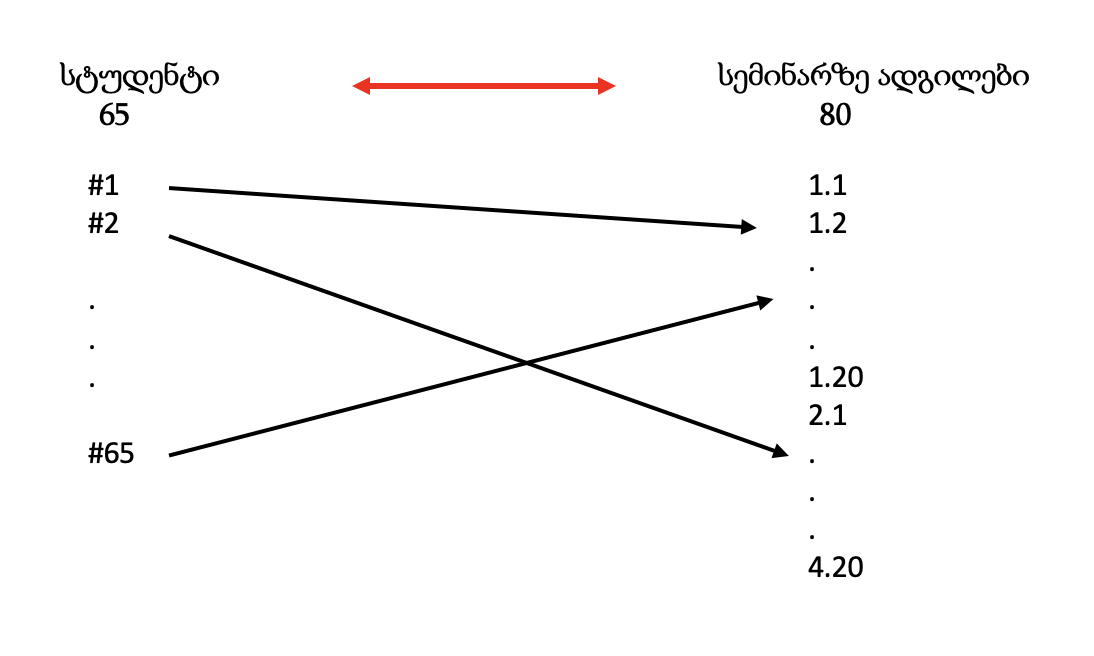
\includegraphics[scale = 0.5]{2.png}
\end{center}

ბ) მოცემული ინფორმაცია არ უზრუნველყოფს იმას, რომ დაწყვილება ყოველთვის იარსებებს. მოვიყვანოთ კონტრმაგალითი: პირველ 21 სტუდენტს აწყობს მხოლოდ პირველი სემინარის დრო. ეს პირობას არ ეწინააღმდეგება, მაგრამ სემინარზე მხოლოდ 20 ადგილია, 1 დაგვრჩება დაუწყვილებელი. მეტიც, პირობას ისიც კი არ ეწინააღმდეგება, რომ 65-ვე სტუდენტს მაგ. მხოლოდ მე-3 სემინარის დრო აწყობდეს, ამ შემთხვევაშიც შეუძლებელია დაწყვილება.

\section{კონსპექტის ამოცანა 10.27(გვ.205)}

ავიღოთ ჩვეულებრივი 52 კარტიანი დასტა და ჩავატაროთ შემდეგი "ფოკუსი". მეგობარს ვთხოვოთ დაალაგოს კარტები მართკუთხედში 4 რიგად და 13 სვეტად, ნებისმიერი მიმდევრობით, რომელიც მას უნდა. შემდეგ ჩვენ ამოვარჩევთ თითო სვეტიდან თითო კარტს ისე, რომ ყველა მნიშვნელობას $(A, 2, 3,\dots 10, J, Q, K)$ თითო კარტი გვეყოლება. ამ ამოცანაში ჩვენი მიზანია დავამტკივოთ, რომ ამის გაკეთება ყოველთვის შეგვეძლება რა მიმდევრობითაც არ უნდა დაალაგოს მეგობარმა კარტები.

ა) აჩვენეთ, როგორ შეიძლება ამ ამოცანის გადაყვანა ორნაწილიან გრაფში დაწყვილების პოვნის ამოცანაზე. აკმაყოფილებს თუ არა თქვენი გრაფი მარტივ კრიტერიუმს, რომ ერთ-ერთ მხარეს მდებარე ყველა წვეროს ხარისხი მეტი ან ტოლია მეორე მხარეს მდებარე ყველა წიბოს ხარისხზე?

ბ) აჩვვენეთ, რომ ნებისმიერ $n$ სვეტში მინიმუმ $n$ სხვადასხვა მნიშვნელობის კარტი დევს და შესაბამისად, დაამტკიცეთ, რომ დაწყვილების თეორემის თანახმად ეს ფოკუსი "გამოვა".

{
\addfontfeatures{FakeBold}
ამოხსნა:
}

ა) $(A, 2, 3,\dots 10, J, Q, K)$-ს ვუწოდოთ კარტის ღირებულება. მოცემული ამოცანა იგივეა, რაც ვიპოვოთ დაწყვილება სვეტის ნომერსა და კარტის ღირებულებას შორის. სვეტი შეგვიძლია დავაწყვილოთ იმ ღირებულებებთან, რომლებიც მასში დევს. თუ ვიპოვით დაწყვილებას, გამოვა რომ გვაქვს ყველა სვეტიდან 1 კარტი არჩეული, და საბოლოო ჯამში ყველა ღირებულების კარტი გვექნება.
თითო სვეტში მინ. 1 და მაქს. 4 განსხვავებული ღირებულების კარტი დევს, თითოეული ღირებულების კარტიც მინ. 1 და მაქს. 4 სვეტში დევს. შესაბამისად, გრაფის ორივე ნაწილში $1 \leq d \leq 4$. ვერ ვიტყვით ერთი ნაწილის $d_{min}$ არის თუ არა $\geq$ მეორე ნაწილის $d_{max}$-ზე. ანუ ჩვენი გრაფი არ აკმაყოფილებს მარტივ კრიტერიუმს, თუმცა ეს არ ნიშნავს, რომ დაწყვილება არ არსებობს.

ბ) ავიღოთ $k$ ცალი სვეტი $(\#a_1,\#a_2, \dots, \#a_k)$ და $l$ რიცხვი $(\#b_1,\#b_2, \dots, \#b_l)$, რომელთანაც ეს სვეტები არიან დაკავშირებულები. $k$ ცალ სვეტში არის $4k$ ადგილი, და $4k$ ადგილზე არ შეიძლება $k$-ზე ნაკლები განსხვავებული ღირებულების კარტი იყოს განლაგებული. ( $k - 1$ ღირებულებაც რომ იყოს $4(k - 1)$ კარტი გვექნება და $4k$ ადგილი ვერ შეივსება). ანუ ამ $k$ ცალ სვეტში მინიმუმ $k$ სხვადასხვა ღირებულების კარტი გვაქვს.
\\გამოდის, რომ ნებისმიერ $k$ ცალ სვეტში მინიმუმ $k$ სხვადასხვა ღირებულების კარტია, სრულდება ჰოლის კრიტერიუმი $\forall S : |N(S)| \geq |S|$, ანუ დაწყვილება ყოველთვის იარსებებს, ფოკუსი "გამოვა".

\begin{figure}[h]
\begin{subfigure}
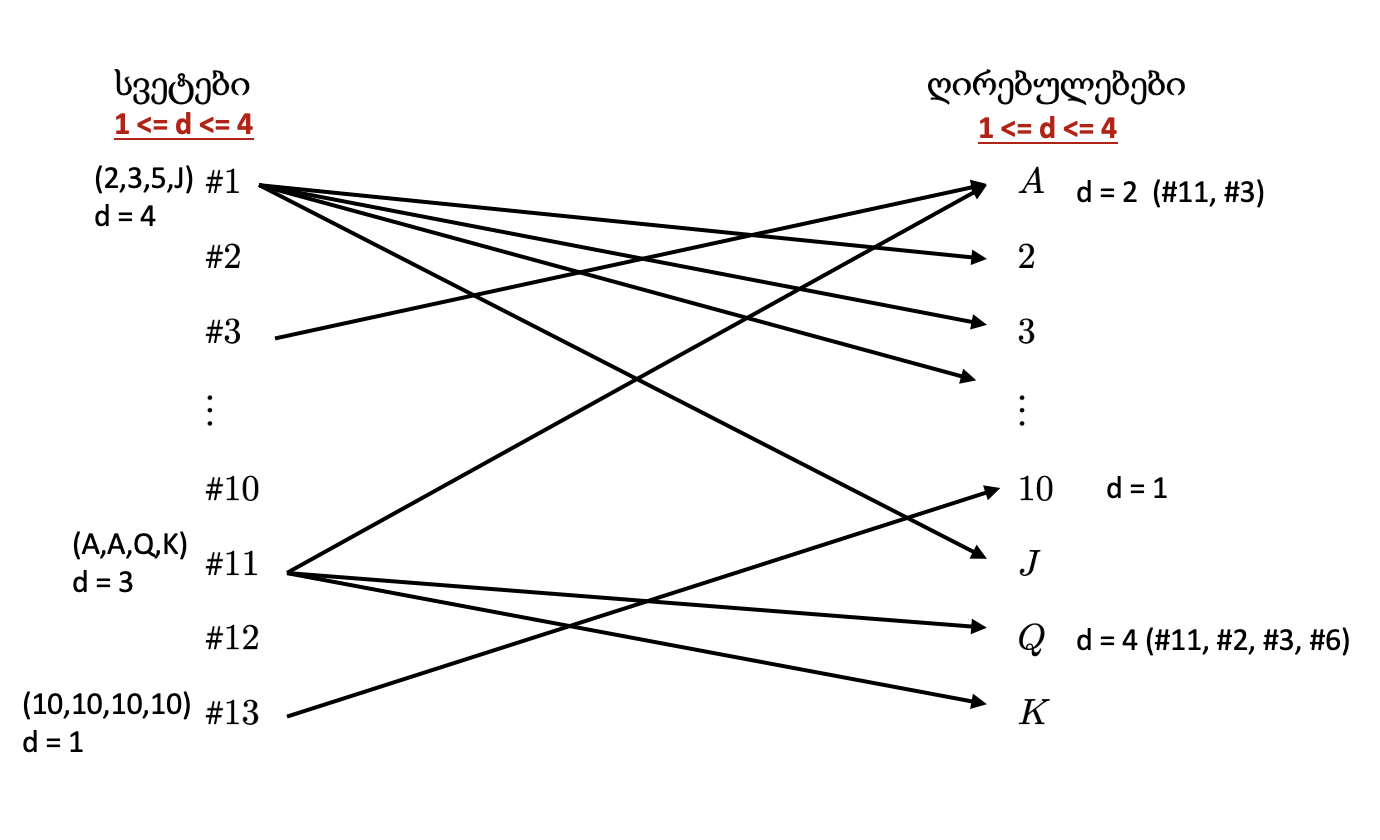
\includegraphics[scale = 0.4]{3.1.png}
\end{subfigure}
\begin{subfigure}
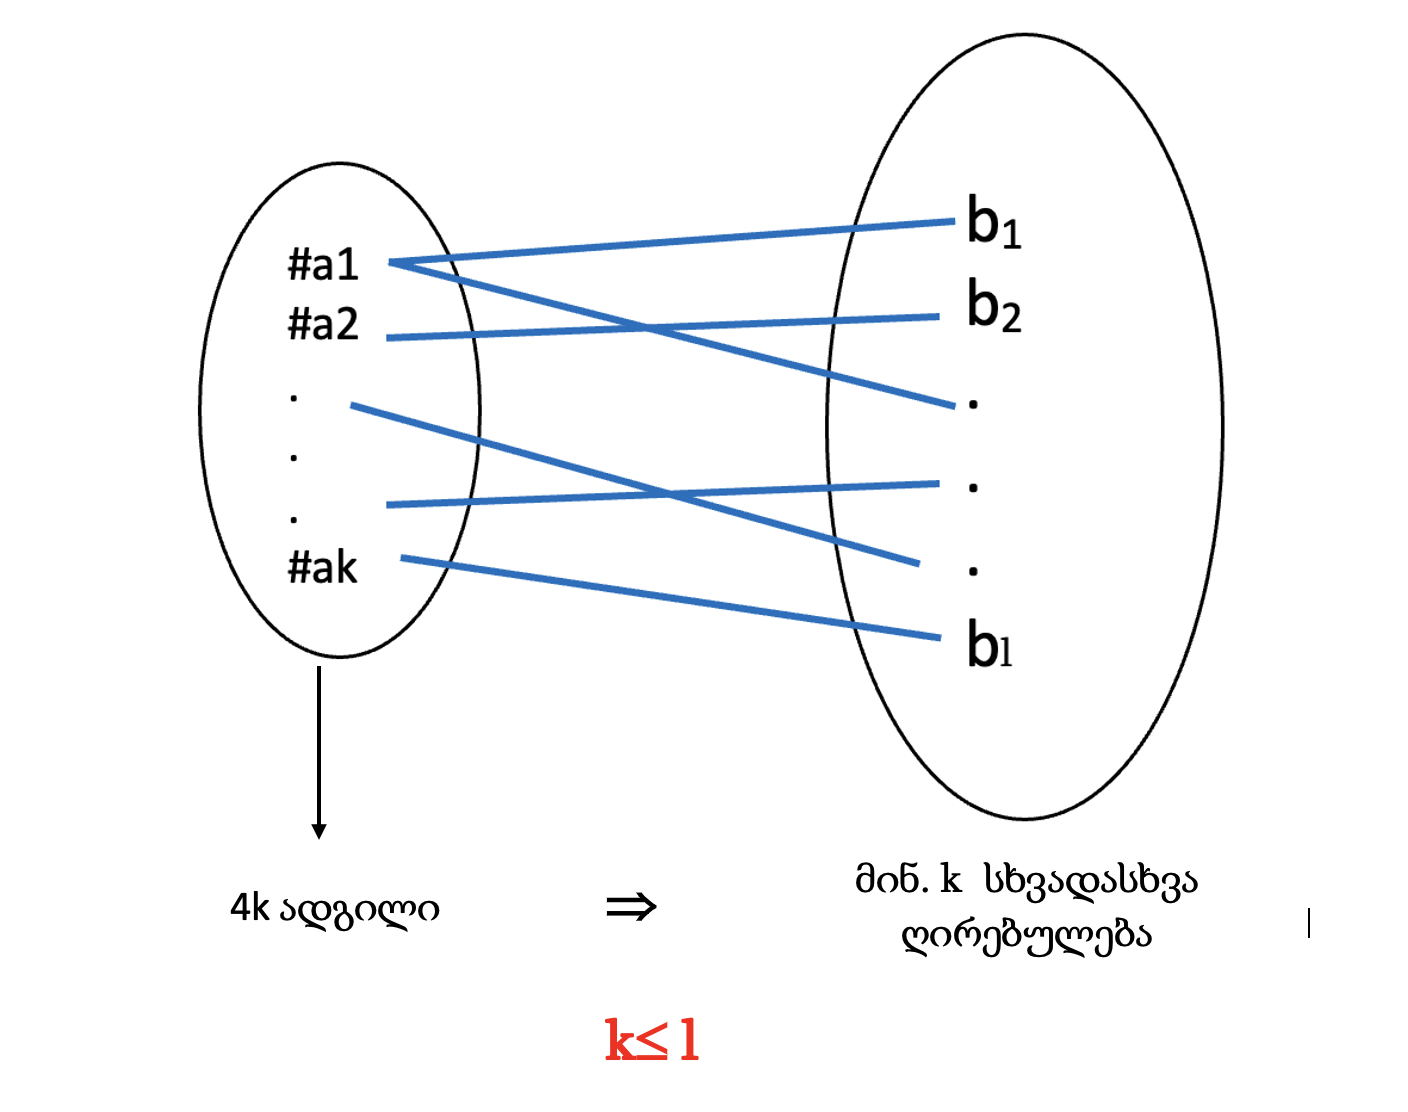
\includegraphics[scale = 0.3]{3.2.png}
\end{subfigure}
\end{figure}

\section{კონსპექტის ამოცანა 10.28(გვ.205)}

სულ განვიხილოთ 20 დადებითი ჩვევა, რომელიც სტუდენტს შეიძლება ჰქონდეს. სემესტრის დასაწყისში ყოველ სტუდენტს ამ 20 ჩვევიდან ზუსტად 8 ცალი აქვს. ყოველი სტუდენტი უნიკალურია, ანუ თუ ერთ სტუდენტს აქვს კონკრეტული 8 ჩვევა, სხვა სტუდენტს ზუსტად იგივე ჩვევბის სიმრავლე არ ექნება. სემესტრის განმავლობაში თითოეულ სტუდენტს უნდა ვასწავლოთ ერთი ცალი ახალი ჩვევა (არ არის აუცილებელი ყველა სტუდენტს ერთი და იგივე ჩვევა ვასწვლოთ).

დაამტკიცეთ, რომ შესაძლებელია სტუდენტებს ისე ვასწავლოთ ჩვევები, რომ სემესტრის ბოლოსაც, როცა ყველა სტუდენტს 9 ჩვევა ექნება, ყველა სტუდენტი ისევ უნიკალური იყოს.

მინიშნება: ეცადეთ ეს ამოცანა ორნაწილიან გრაფში დაწყვილების პოვნის ამოცანაზე დაიყვანოთ. ერთ და მეორე მხარეს წვეროებად რა უნდა აიღოთ რთული მისახვედრია და თუ პირველივე ცდაზე არ გამოგივიდათ, სხვადასხვა ვარიანტების სცადეთ. საბოლოო ჯამში ისეთ გრაფს მიიღებთ, რომლის ერთ ნაწილში მყოფი წვეროების ხარისხი მეორე ნაწილში მყოფი წვეროების ხარისხებზე ყოველთვის მეტია.

{
\addfontfeatures{FakeBold}
ამოხსნა:
}

სტუდენტები ანუ მათი 8 ჩვევიანი სიმრავლეები და 9 ჩვევიანი სიმრავლეები ანუ მათი შესაძლო მომავლები დავაწყვილოთ, ანუ ჩვენი ამოცანა დავიყვანეთ ორნაწილიან გრაფში დაწყვილების პოვნის ამოცანაზე. თითოეული სტუდენტი შეიძლება დაწყვილდეს ისეთ, მომავალთან რომელიც შეიცავს ამ სტუდენტის 8 ჩვევას და მე-9 განსხვავებული იქნება ის ჩვევა, რომელსაც ეს სტუდენტი ამ სემესტრში ისწავლის. თუ ასეთ დაწყვილებას ვიპოვით, სემესტრის ბოლოსაც უნიკალურები იქნებიან სტუდენტები, რადგან თითოეულს დავუწყვილეთ უნიკალური 9 ჩვევიანი კომბინაცია. 
\begin{center}
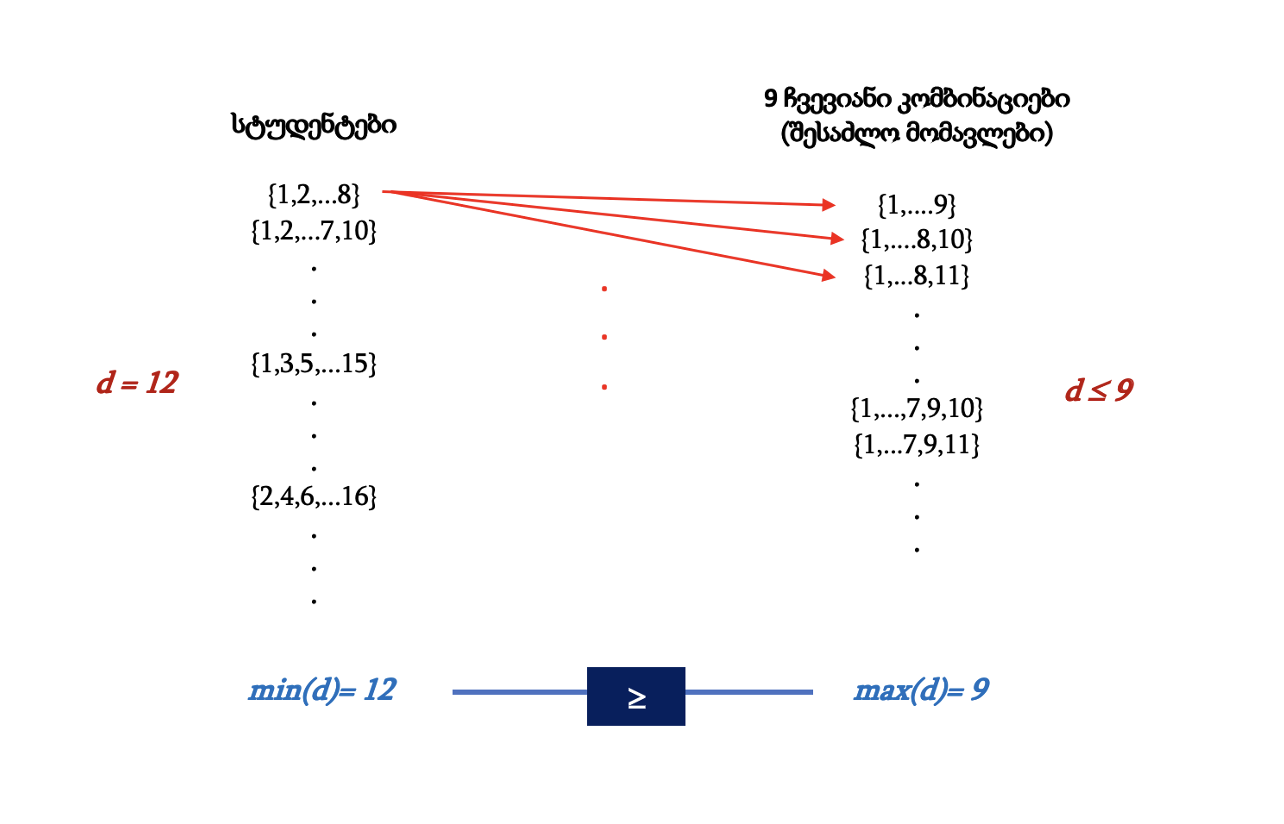
\includegraphics[scale = 0.7]{4.png}
\end{center}
\\ თითოეულ სტუდენტს 8 ჩვევა აქვს, სულ 20 ჩვევაა, ანუ ამ სემესტრში სტუდენტმა შეიძლება ისწავლოს დარჩენილი 12-დან ნებისმიერი, ანუ აქვს 12 შესაძლო მომავალი.
ყველა სტუდენტის წვეროს ხარისხი $d = 12$. 
\\ თითოეული 9 ჩვევიანი კომბინაცია შეიძლება დაუკავშირდეს იმ სტუდენტებს, რომლის 8 ჩვევა შედის ამ 9 ჩვევიან სიმრავლეში ანუ ისეთ 8 ჩვევიან სიმრავლეებს, რომელიც ამ 9 ჩვევიანი სიმრავლის ქვესიმრავლეა. დავთვალოთ ასეთი ქვესიმრავლეების რაოდენობა: $\binom{9}{8} = \frac{9!}{8!(9-8)!} = 9$.
\\  თითოეული 9 ჩვევიანი კომბინაცია შეიძლება დაუკავშირდეს 9 სტუდენტს, თუმცა არ არის აუცილებელი ყველა 9 ჩვევიანი კომბინაციას შეესაბამებოდეს სტუდენტს, მთავარი ყველა სტუდენტი დაწყვილდეს შესაძლო მომავალთან. ამიტომ შესაძლო მომავლების $d \leq 9$.
\\ ამ ორნაწილიანი გრაფის მარცხენა მხარის (სტუდენტების) $d_{min} = 12$, მარცხენა მხარის (შესაძლო მომავლების) $d_{max} = 9$.
\\ ერთი ნაწილის $d_{min}$ $\geq$ მეორე ნაწილის $d_{max}$, მარტივი კრიტერიუმის თანახმად, დაწყვილება შესაძლებელია.
\\ შესაბამისად, შესაძლებელია სტუდენტებს ისე ვასწავლოთ ჩვევები, რომ სემესტრის ბოლოსაც, როცა ყველა სტუდენტს 9 ჩვევა ექნება, ყველა სტუდენტი ისევ უნიკალური იყოს.

\end{sloppypar}
\end{document}
